\section{Strimzi system tests}
\label{02:sec:strimzisystemtests}

This Section describes the basics of the Strimzi system tests.
We start with a short description of how we test the Strimzi product.
Then in the section \ref{02:subsec:strimziJunit5relation:execution} we explain the fundamentals of JUnit5, how tests are discovered and executed. Lastly, in Section \ref{02:subsec:strimzisystemtestsexecution} we explain Strimzi system test management and execution flow. 

It all starts with a regression, where we begin with unit tests, integration tests, and system tests. Of course, the most time-consuming is system tests, which in our case take about 40 hours. 
\begin{figure}[!ht]
    \centering
    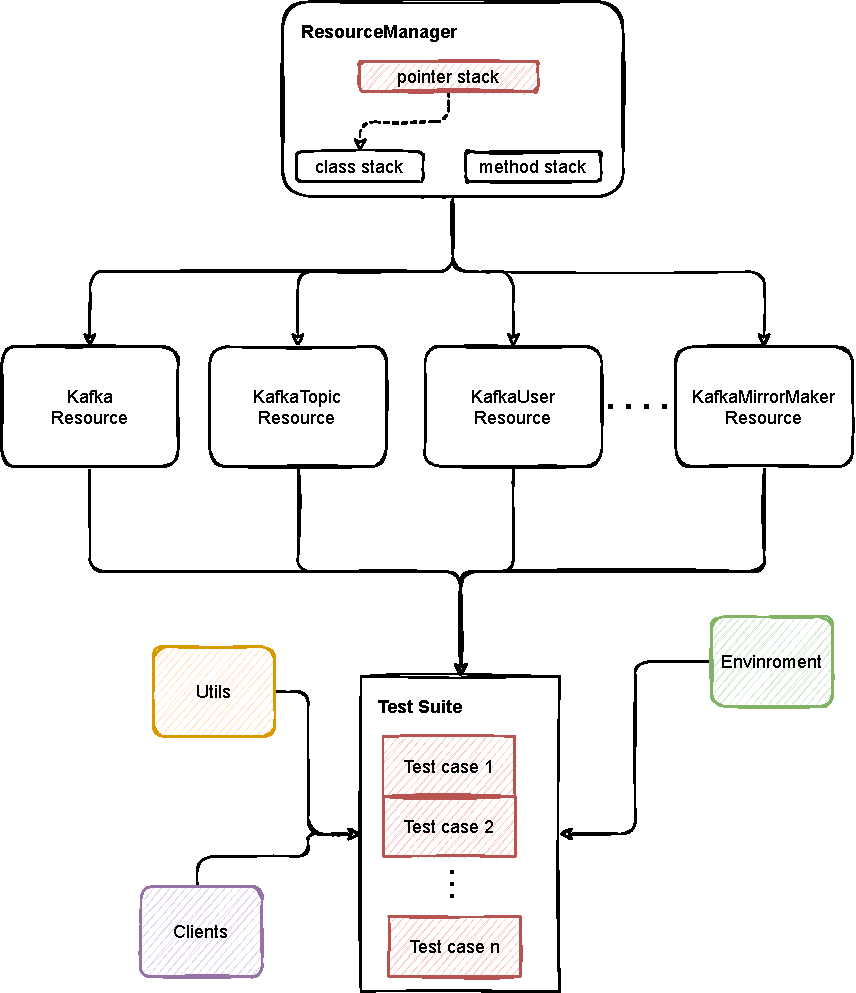
\includegraphics[scale=0.80]{obrazky-figures/02-preliminaries/04-strimzi-system-tests/01-architecture-overall.pdf}
    \caption{Strimzi system tests top-level component architecture}
    \label{02d:fig:strimzisystemtestarch}
\end{figure}
The testing phases are dependent on each other in the order in which they are executed. For instance, integration tests will not run if unit tests fail, similarly for integration and system tests. Furthermore, system tests run on multiple infrastructures such as Openstack, Microsoft Azure or Amazon Web Services. On each of these infrastructures, there are certain limitations for the set of tests. Since these are Kubernetes system tests, it is essential to realize that the total load on the resource is enormous. At the same time, the preparation of resources and their cleaning is time-consuming. Therefore, our system tests have two essential parts. The first is resource classes that provide the user interface for creating, retrieving, deleting, and updating these resources.
Moreover, we have three stacks that take care of the total test case lifecycle. These stacks are responsible for storing all resources based on the test case. Furthermore, the deletion of these resources is transparent for the user as well as if it is a resource created in \emph{@BeforeAll}\footnote{\textbf{@BeforeAll } \---\ is JUnit5 annotation, where one specify what must be executed before all tests in the test suite.} annotation. The second fundamental part is auxiliary classes such as Utils \footnote {\textbf{Utils} \---\ type of class that consists of static methods, which in general dynamically waiting for a specific event. For instance, waiting for Rolling Update, if one change Kafka configuration}, Apache Kafka clients for external communication, Kubernetes client offering an API for communication with the Kubernetes cluster and finally classes such as Constants and Environment. This can be seen in Figure \ref{02d:fig:strimzisystemtestarch}.

\subsection{JUnit5 relation and execution of test cases}
\label{02:subsec:strimziJunit5relation:execution}

The entire implementation and management of the test lifecycle are in charge of Junit5 Engine. The Engine facilitates the discovery and execution of tests for a specific programming model. In other words, it is the entity in charge of discovering and executing tests. Discovering can be thought of as a scan of all the classes and methods in specific directories. The Engine has specified in advance which signatures to include in the test tree. In the case of the Junit5 Engine, it is a sequence of chaining methods, which gradually add all classes (test suites) and methods (test cases) to the test tree. They also add the test types defined by them (i.e., \emph{@TestFactory}, \emph{@ParametrizedTest}, \emph{@TestTemplate}). Everything can be seen in the  Algorithm \ref{02:alg:selectorresolver}. 

\begin{algorithm}[H]
    \label{02:alg:selectorresolver}
    \caption{Junit5 Engine: Discovery selector resolver}
    \begin{algorithmic}[1]
        \Procedure{resolveSelectors}{DiscoveryRequest request, Descriptor descriptor}
        \State {EngineDiscoveryRequestResolver.$<$JupiterEngineDescriptor$>$builder()}
		\State {.addClassContainerSelectorResolver(new IsTestClassWithTests())}
		\State {.addSelectorResolver(c $\rightarrow$ new ClassSelectorResolver(classFilter, config))}
		\State {.addSelectorResolver(c $\rightarrow$ new MethodSelectorResolver(config))}
		\State {.addTestDescriptorVisitor(c $\rightarrow$ new ClassOrderingVisitor(config))}
		\State {.addTestDescriptorVisitor(c $\rightarrow$ new MethodOrderingVisitor(config))}
		\State {.addTestDescriptorVisitor(c $\rightarrow$ TestDescriptor::prune)}
		\State {.build();}
		\State {.resolve(request, descriptor);}
		\EndProcedure
    \end{algorithmic}
\end{algorithm}

Once the resolver is created, we can run the following algorithm, using the resolver and creating the already mentioned tree of \emph{TestDescriptors}. Here is a detailed description of how the algorithm works:

\begin{enumerate}[itemsep=1mm, parsep=0pt]
    \item Enqueue all selectors in the supplied request to be resolved.
    \item While there are selectors to be resolved, get the next one. Otherwise, the resolution is finished.
    \begin{enumerate}
        \item Iterate over all registered resolvers in the order they were registered in and find the first one that returns a resolution other than unresolved().
        \item If such a resolution exists, enqueue its selectors.
        \item For each exact match in the resolution, expand its children and enqueue them as well.
    \end{enumerate}
    \item Iterate over all registered visitors and let the engine test descriptor accept them.
\end{enumerate}

The second phase after the correct scan of test cases that the user wants to perform is execution. In this case, TestEngine already has a TestDescriptor in which all the information needed to run is available. At this stage, the TestEngine must always notify the Junit5 platform of the success or failure of the test case. Moreover, Engine instantiates the \emph{SameThreadHierarchicalTestExecutorService} class, which ensures that each test is performed sequentially.

\subsection{Strimzi system test management and execution flow}
\label{02:subsec:strimzisystemtestsexecution}

In the previous Section \ref{02:subsec:strimziJunit5relation:execution}, we described the intricate parts of loading and the type of tests performed. In the case of the Strimzi part, it is necessary to add several mechanisms (i.e., creation of Kubernetes cluster, communication with Kubernetes cluster, management of Kubernetes resources, wait for conditions). We solve all these parts in Strimzi. We have created a Kubernetes cluster in several ways, as we test the product on several infrastructures. For example, on Microsoft Azure, we create a Minikube (a subset of the Kubernetes cluster, one-node cluster) with approximately eight CPUs and 16GB of RAM. In Openstack, we typically create a six node cluster consisting of three master nodes and three worker nodes. Each of them has eight CPUs and 16GB available (similarly to Amazon Web Services).

Communication with the Kubernetes cluster is guaranteed by the Kubernetes client \url {https://github.com/fabric8io/kubernetes-client}. This client provides a large number of methods that communicate directly via the Kubernetes REST API. Most of the methods are designed to create, update, delete and retrieve a given resource. In practice, we will also encounter the term CRUD methods. To illustrate, we can imagine getting all the namespaces on a given Kubernetes cluster. All namespaces are obtained using the command \emph{client.namespaces().List();}.

\begin{algorithm}[H]
    \label{02:alg:deletionalg}
    \caption{ResourceManager generic deletion algorithm}
    \begin{algorithmic}[1]
        \Procedure{deleteLater}{MixedOperation$<$T, ?, ?, ?$>$ operation, T resource}
        \State switch(resource.getKind()) \{
        \State \hspace{2em} case Kafka.RESOURCE\_KIND$:$
        \State \hspace{4em} pointerResources.push(() $\rightarrow$ {
        \State \hspace{4em} operation.inNamespace(resource.getMetadata().getNamespace())
        \State \hspace{4em} .withName(resource.getMetadata().getName())
        \State \hspace{4em} .withPropagationPolicy(DeletionPropagation.FOREGROUND)
         \State \hspace{4em} .delete();
         \State \hspace{4em} waitForDeletion((Kafka) resource);
         \State \hspace{2em} });
        \State \hspace{2em} break;
        \State \hspace{2em} case KafkaConnect.RESOURCE\_KIND$:$
        \State \hspace{2em} case KafkaMirrorMaker.RESOURCE\_KIND$:$
        \State \hspace{2em} \dots (other resource)
        \State \hspace{4em} // similar to Kafka resource
        \State \hspace{2em} default:
        \State \hspace{4em}        pointerResources.push(() $\rightarrow$  {
         \State \hspace{4em}           operation.inNamespace(resource.getMetadata().getNamespace())
         \State \hspace{4em}                   .withName(resource.getMetadata().getName())
          \State \hspace{4em}                  .withPropagationPolicy(DeletionPropagation.FOREGROUND)
          \State \hspace{4em}                  .delete();
           \State \hspace{2em}     });
           \State \}
           \State return resource;
		\EndProcedure
    \end{algorithmic}
\end{algorithm}
The overall orchestration of Kubernetes resources is handled by the \emph{ResourceManager} class and its additional resource classes. As we wrote at the beginning of the \ref{02:sec:strimzisystemtests} Section, it includes three stacks and where the main/pointer stack points to method or class stack based on context. For example, suppose the execution is located in \emph{@BeforeAll} or \emph{@AfterAll} annotation, we add elements to the class stack. In other scenarios, such as in the test case or \emph{@BeforeEach}, we add elements to the method stack. This data structure will guarantee the correct order of deleting resources at the end of each test or test class. This is because we want to delete resources in the order they were created. So if we create first Kafka, Producer and lastly Consumer, then in the clean-up phase, we will first delete Consumer, Producer and finally Kafka. Thus, the user who creates the test cases does not have to delete individual resources created for the entire test. In other words, the clean-up phase is transparent to the user. However, if one wants to explicitly delete the resource, it is possible via the following command \emph{ResourceType.delete(name)}. Algorithm \ref{02:alg:deletionalg} defines clean-up phase.


By contrast, when creating any resources, the user has at his disposal, for example, KafkaResource, KafkaTopicResource and the like. Each of these classes contains predefined templates that include specific configuration settings. A typical example is Kafka, which can be seen by \ref{02:fig:kafkaresource:defaultmethod}.

\begin{figure}[!ht]
\begin{lstlisting}
private static KafkaBuilder defaultKafka(Kafka kafka,
            String name, int kafkaReplicas, int zookeeperReplicas) {
    return new KafkaBuilder(kafka)
        .withNewMetadata()
            .withName(name)
            .withNamespace(ResourceManager.kubeClient().getNamespace())
        .endMetadata()
        .editSpec()
            .editKafka()
                .withVersion(Environment.ST_KAFKA_VERSION)
                .withReplicas(kafkaReplicas)
            .endKafka()
            .editZookeeper()
                .withReplicas(zookeeperReplicas)
            .endZookeeper()
            .editEntityOperator()
                .editUserOperator()
                    .withNewInlineLogging()
                        .addToLoggers("rootLogger.level", "DEBUG")
                        .endInlineLogging()
                .endUserOperator()
                .editTopicOperator()
                    .withNewInlineLogging()
                        .addToLoggers("rootLogger.level", "DEBUG")
                    .endInlineLogging()
                .endTopicOperator()
            .endEntityOperator()
        .endSpec();
}
\end{lstlisting}
    \caption{Default Kafka Custom Resource in KafkaResource.class}
    \label{02:fig:kafkaresource:defaultmethod}
\end{figure}

Another part of the Strimzi system tests is the wait for methods mechanism. It is used primarily in scenarios where it is necessary to wait for an event to occur. An example could be waiting for a Rolling Update to occur when Kafka's original Statefulset changes. \begin{figure}[!ht]
    \centering
    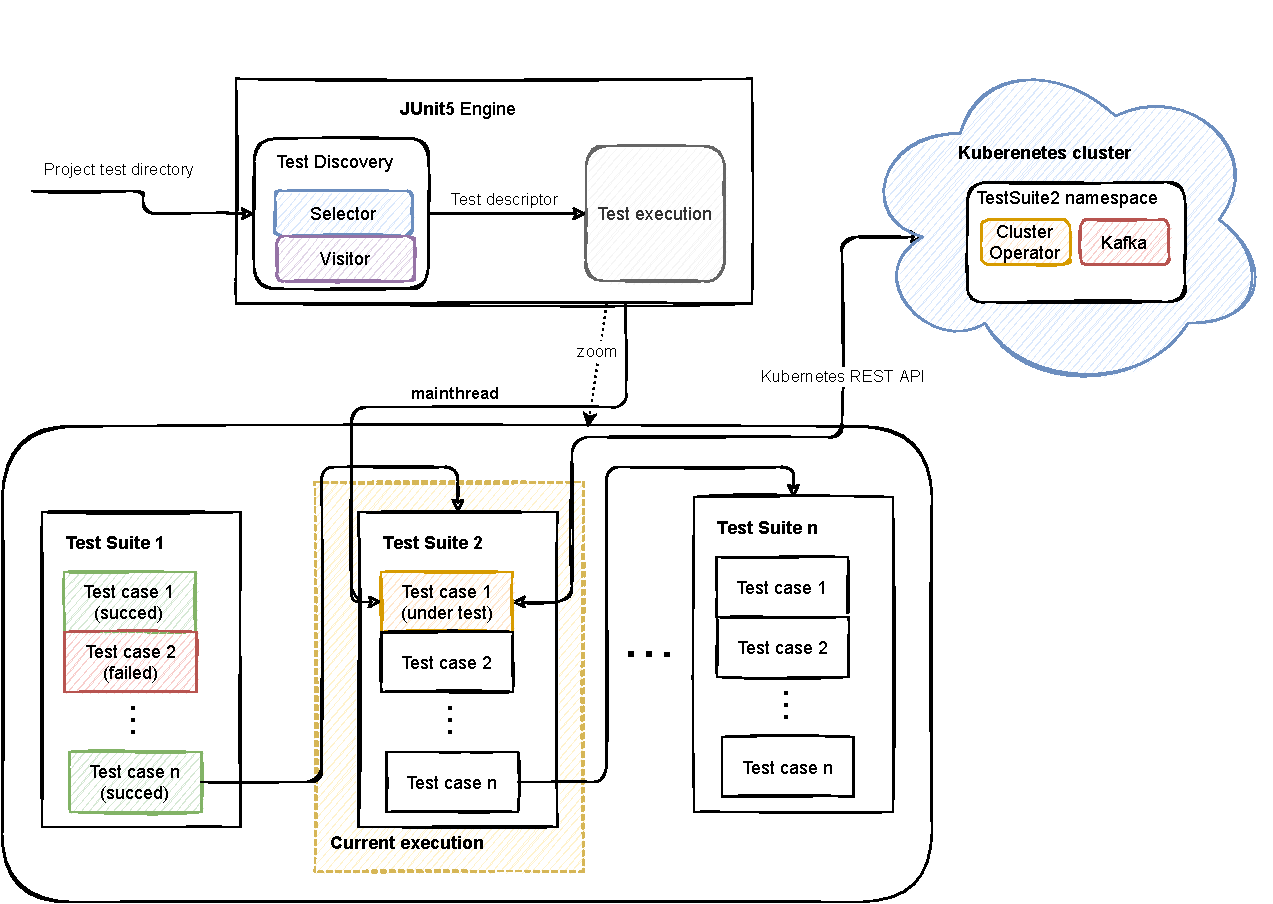
\includegraphics[scale=0.70]{obrazky-figures/02-preliminaries/04-strimzi-system-tests/02d-strimzisystemtest-sequence-execution.pdf}
    \caption{Strimzi system tests execution flow}
    \label{02d:fig:strimzisysmtetest:execution}
\end{figure}
The second example could be while waiting for a particular pessimistic scenario (i.e., the Cluster Operator Pod will switch to the CrashLoopBack state, the KafkaBridge Deployment Status will contain the text in the message).

So if we summarize everything we have learned. It all starts with scanning the test directory, which provides a tree of TestDescriptors. This is the primary responsibility of TestEngine, which uses selectors to filter out all test cases and the visitors who accept the individual test cases. As soon as we have a tree available, which consists of TestDescriptor nodes, TestEngine starts execution. This execution is sequential for each test case. At the same time, thanks to our management and defined resources, we can communicate with the Kubernetes cluster. For example, in Figure \ref{02d:fig:strimzisysmtetest:execution} we can execute n the number of Test suites where Test Suite 2 is currently executed and specifically Test Case 1. The attentive reader will somehow realize that the overall execution model is sequential due to Java's main thread, the primary thread identifier.